% -*- coding: utf-8; ispell-dictionary: "french"; -*-

\documentclass[11pt]{report}

\usepackage{graphicx}
\graphicspath{{img/}}
\usepackage[utf8]{inputenc}
\usepackage[francais]{babel}
\usepackage[T1]{fontenc}
\usepackage{alltt}
\usepackage{xcolor}
%\usepackage{amssymb}
\usepackage{multicol}
\usepackage{geometry}
%% \usepackage{amsfont}
\usepackage{amsmath}
\usepackage{amssymb}
\usepackage{url}
\usepackage[toc,page]{appendix}
\geometry{left=23mm, right=23mm, top=30mm, bottom=25mm}

\newcommand{\bcode}[1]{\textcolor{darkgray}{#1}}
\renewcommand{\ttdefault}{txtt}

\newcommand{\cercles}{CERCLES$^2$ }


\usepackage{fancyhdr}
\pagestyle{fancy}
\lhead{\textsc{Rapport de stage}}
\rhead{\textsc{Florian Thibord}}


\title{
	\normalsize{M2 Informatique STL APR\\
	Université Pierre et Marie Curie\\
	2012-2013}\\
	\vspace{3mm}
	\rule{\linewidth{}}{0.3mm}\\
	\Large{Rapport de Stage}\\
	\Large{Traduction de composants Scade/Lustre vers des machines B}\\
	\vspace{3mm}
	\normalsize{Florian THIBORD}
	\rule{\linewidth{}}{0.3mm}
}

\author{}

\date{}

\setcounter{tocdepth}{1}

%----------------------------------
%-------- DEBUT DOCUMENT ----------
%----------------------------------

\begin{document}

\maketitle
\clearpage

\tableofcontents 
\newpage

\chapter*{Introduction}
% -*- coding: utf-8; ispell-dictionary: "french"; -*-

%--------------
% Introduction
%--------------


Ce stage s'est déroulé au sein du projet ANR-10-SEGI-017 \cercles\cite{Cercles}.
L'objectif du projet est de certifier formellement
des composants réutilisables, afin de réduire les tests en prouvant
grâce à des méthodes formelles la sûreté des différentes briques formant un
logiciel. L'intérêt est à la fois pratique par la réutilisabilité des composants
certifiés, et économique en réduisant le temps et le coût des tests. \\  

Un acteur majeur du développement de systèmes embarquées critiques est Scade,
un acronyme pour Safety Critical Application Developpement Environment. Cet
environnement de développement est basé sur la programmation graphique, par
schémas-blocs, permettant de définir des programmes faciles à lire et
d'engendrer du code compilable (C ou ADA). Il est 
notamment utilisé en aéronautique (grande partie du logiciel embarqué de
l'A380), dans le domaine spatial ou dans le nucléaire. Dans le cadre du projet,
les composants sont écrits soit avec Scade, soit avec un environnement de
développement similaire, Simulink. Cependant, il est possible d'importer des
composants Simulink dans l'environnement Scade. \\

%% \begin{figure}[h]
%% \begin{center}
%% 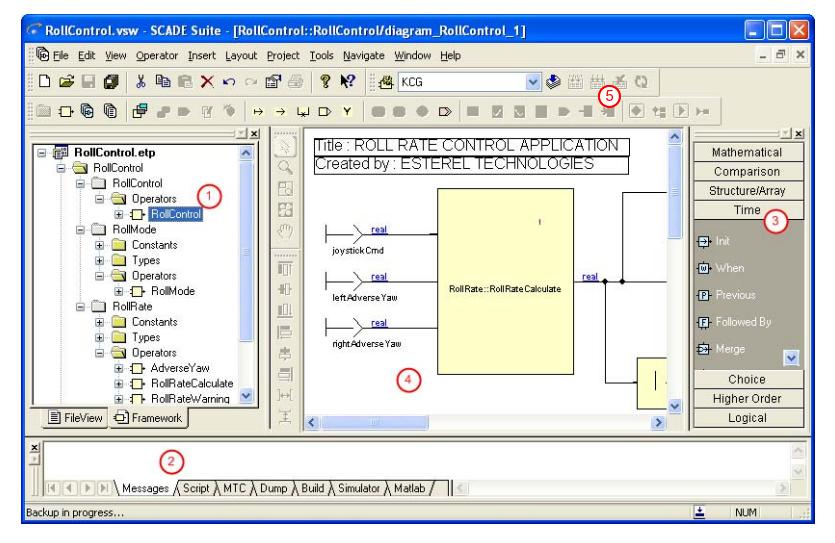
\includegraphics[scale=0.36]{intro_scade_pic.jpg}
%% \end{center}
%% \caption{Capture d'écran de l'envioronnement Scade}
%% \end{figure}

Pour assurer que ces composants et leur réutilisation sont sûrs, on
utilise une méthode formelle, qui permet d'exprimer la signification d'un
composant dans un formalisme mathématique, afin de démontrer leur
validité par rapport à une spécification.\\
Il faut alors introduire le concept des \emph{contrats}: un contrat est
associé à un composant et indique des conditions sur ses entrées
(pré-conditions) et sur ses sorties (post-conditions). Ils formeront
ainsi une spécification du composant. 
A la fin des années 60, C.A.R Hoare donne la définition suivante \cite{Hoare} : Soit $P$ et
$R$ les pré-conditions et post-conditions associées au programme $Q$, \\
%% \noindent
%% \fbox{
\begin{minipage}{\textwidth}
\begin{center}
$P\{Q\}R$ \\
\emph{"If the assertion P is true before initiation of a program Q, then the
assertion R will be true on its completion"}
\end{center}
\end{minipage}
%% }
\\
Cette définition donnera une première intuition qui sera reprise par Bertrand
Meyer lorsqu'il introduira la programmation par contrat avec le language Eiffel
en 1985.\\

\noindent
A partir d'un programme et de son contrat, il faut alors vérifier formellement
que: 
\begin{itemize}
\item  (i) Le programme est cohérent vis-à-vis de sa spécification.
\item (ii) l'initialisation du programme satisfait les pré-condition, et en
conséquence de (i) le résultat satisfait les post-conditions.
\end{itemize}
La validation est alors faite par une démonstration formelle.\\

Il existe différentes approches de démonstrations formelles associées aux programmes, comme celle basée
sur des règles de typage, introduites par la correspondance de
Curry-Howard dans à la fin des années 50. 
L'avantage de la méthode choisie, la méthode B, est qu'elle a déjà
fait ses preuves industriellement, elle a notamment été utilisée pour
développer la ligne METEOR (ligne 14) du métro parisien, qui est
entièrement automatisée.\\ 
Elle a été introduite
par J.R. Abrial dans les années 80 \cite{JRA}. Elle est basée sur le \emph{raffinement} de
spécifications formelles vers une spécification exécutable. La spécification
formelle est rédigée dans un formalisme mathématique de haut niveau appelé
\emph{machine abstraite}, dont le principe de calcul est basé sur le calcul
des prédicats du premier ordre étendu avec une théorie des
ensembles. Le raffinement de cette machine abstraite consiste à la
reformuler de façon plus concrète et à l'enrichir avec des
\emph{substitutions} correspondants aux instructions du composant. Le
raffinement de plus bas niveau, exécutable, est appelé \emph{implantation}. Il peut y
avoir des raffinements intermédiaires, mais dans le cadre du projet nous n'aurons besoin que
d'une étape de raffinement, de la machine abstraite vers l'implantation. Chaque
étape de raffinement passe par une étape d'\emph{obligations de preuves}, une
validation par démonstration formelle, garantissant la fidélité de la
machine raffinée par rapport à la machine abstraite. \\

Mon travail fut de développer un traducteur permettant de transposer un
composant écrit en SCADE vers un couple de machines B. \\
Un composant Scade est constitué d'un \emph{noeud}
correspondant à un programme, et d'un ensemble de conditions sur les
entrées et sorties du programme qui vont former le contrat. 
Le traducteur suit une ligne de compilation classique, prenant en
entrée le programme et son contrat, et produit en sortie une machine abstraite
correspondant au contrat, ainsi qu'une machine raffinée qui implante le programme. \\

\begin{figure}[h]
\begin{center}
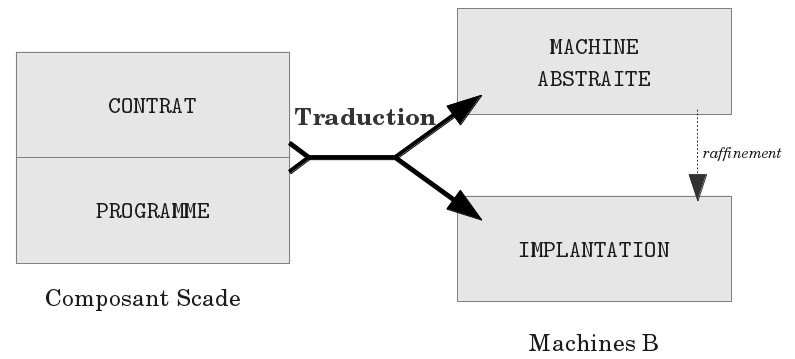
\includegraphics[scale=0.54]{intro_schema2.png}
\end{center}
\caption{Schéma du principe de traduction}
\end{figure}

\addcontentsline{toc}{chapter}{Introduction}

\chapter{Scade}
% -*- coding: utf-8; ispell-dictionary: "french"; -*-

%----------------------------
% Chapter 1 - Fragment Scade
%----------------------------


Scade a été développé par le laboratoire Verimag à partir des travaux sur
le langage synchrone Lustre, puis repris par la société Esterel Technologies \cite{Estech}. On retrouve
ainsi les notions de Lustre dans le langage de Scade, un programme est découpé
en noeuds dont les entrées et sorties sont des \emph{flux de données}. Ces
noeuds sont les composants que nous voulons traduire. 
Les noeuds Scade considérés dans le cadre du projet \cercles  sont
soumis à quelques restrictions. En effet, il faut limiter le langage
utilisé, car certains éléments du langage sont spécifiques aux
langages synchrones et ne sont donc pas traduisibles en B.\\

% SECTION 1 : Présentation

\section{Architecture d'un composant Scade}

\paragraph{}
Scade étant un environnement de programmation par schémas-blocs, on
développe avec des "boîtes". Par exemple, un programme prenant en
entrées 3 entiers \texttt{b\_sup}, \texttt{b\_inf} et \texttt{z}, qui retourne un entier v égal
à:
\begin{itemize}
\item \texttt{z}, si \texttt{z} est compris entre \texttt{b\_inf} et \texttt{b\_sup}
\item \texttt{b\_inf}, si \texttt{z} est inférieur à \texttt{b\_inf}
\item \texttt{b\_sup}, si \texttt{z} est supérieur à \texttt{b\_sup}
\end{itemize}
Ce programme s'écrira de la façon suivante dans Scade. 

\begin{figure}[h]
\begin{center}
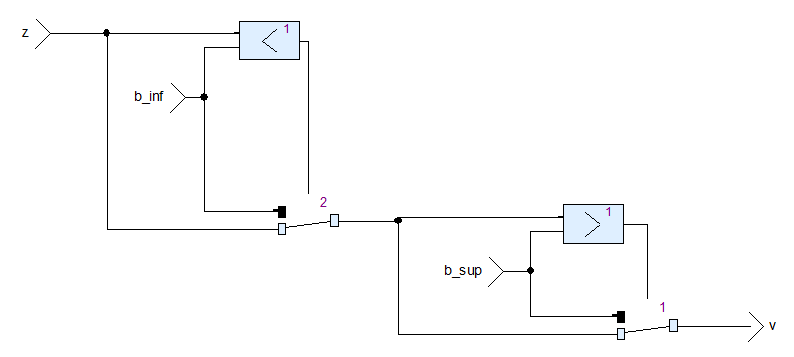
\includegraphics[scale=0.7]{1_bound.png}
\end{center}
\caption{Version graphique du noeud bound}
\end{figure}

La version textuelle de ce programme correspond au noeud \texttt{bound} suivant:

\begin{figure}[h]
\begin{center}
\begin{verbatim}
node bound (z: int; b_inf: int; b_sup: int) returns (v: int);
var
  a: int;
  c1: int;
  c2: int;
let
  a = if c1 then b_inf else z;
  v = if c2 then b_sup else a;
  c1 = z < b_inf;
  c2 = a > b_sup;
tel
\end{verbatim}
\end{center}
\caption{Version tectuelle}
\end{figure}

\paragraph{}
Au niveau des types de données utilisées, on pourra manipuler
des entiers, réels et booléens. On pourra également manipuler des
tableaux de ces types. En revanche, les types définis par
l'utilisateur tels que les types enregistrement ne seront pas gérés
par le traducteur.\\
Le comportement du noeud est ensuite défini par une liste d'équations,
dont l'ordre n'a pas d'importance. Ces équations sont de la forme:
\begin{verbatim}
left_part = expr;
\end{verbatim}
Où \texttt{left\_part} désigne une variable locale ou une sortie du composant, et expr
est une expression portant sur une ou plusieurs variables locales ou entrées.

\paragraph{}
Les expressions disponibles sont toutes les expressions arithmétiques
(\texttt{+, -, /, *, mod}), les expressions relationnelles (\texttt{<, >, <=, >=, =, <>})
et logiques (\texttt{and, or, xor, not}). Sont également disponibles les opérations sur les tableaux, telles que
la définition, l'index, et la concaténation. Lors de la génération
textuelle du noeud, Scade \emph{atomise} l'ensemble des opérations et
introduit des variables locales qui correspondent aux fils du
noeud. Pour ces opérations, la forme des équations sera donc toujours
semblable, on aura une seule variable à gauche de l'équation, et à
droite, on aura un opérateur appliqué à un ensemble de variables:

\texttt{v = op$_{base}$(x$_1$, ..., x$_n$);}\\
Les expressions conditionelles sont également possibles:

\texttt{v = if c then x$_1$ else x$_2$;}\\
avec \texttt{c}, \texttt{x$_1$} et \texttt{x$_2$} des variables. 

Enfin, on peut évidemment faire des appels à d'autres
noeuds, pour mettre en pratique la notion de composant
réutilisable. Les équations correspondantes peuvent avoir plusieurs
variables dans la partie gauche de l'équation, car un noeud appelé
peut avoir plusieurs sorties.

\texttt{v$_1$, ..., v$_p$ = op$_{appel}$(x$_1$, ..., x$_n$);}



% SECTION 2 : Restrictions

\section{Le temps avec Scade}

Le temps est un élément primordial dans ces systèmes dits "réactifs", où
l'on manipule des flux de données. Le temps est discrétisé en instants,
et chaque instant correspond à 1 tic de l'horloge de base. A chaque
instant i, les équations du noeud sont résolues à partir du flux reçu
en entrée à cet instant, et produit le flux de sortie correspondant au
résultat au même instant.

\paragraph{Une horloge unique}
Avec les langages synchrones, on peut
synchroniser des instructions sur des horloges différentes. On utilise des
opérateurs spécifiques au temps pour synchroniser une instruction sur une
horloge spécifique. Pour assurer la bonne définition des noeuds dont les
instructions sont calculées sur des horloges différentes, il existe
une étape de calcul des horloges \cite{Pouzet}.
Cependant, dans le cadre de ce projet, nous n'utiliserons qu'une seule horloge,
celle de base. Toutes les équations sont résolues au même instant. 

\paragraph{L'opérateur fby}
Il y a un seul opérateur temporel qui reste utilisable, c'est
l'opérateur \texttt{fby}. Cet opérateur prend 3 arguments:
\begin{itemize}
\item une variable v
\item un délai
\item une initialisation
\end{itemize}
A l'instant i\footnote{On suppose que le premier instant est l'instant
0}, \texttt{fby} retourne la valeur de la variable v à
l'instant (i - délai). Dans le cas ou (i - délai) est négatif,
l'opérateur retourne la valeur initialisation.
Par exemple, on représente dans le tableau suivant la valeur de sortie
de l'opérateur \texttt{fby} en fonction de la valeur d'une variable
d'entrée \texttt{v}, avec une initilisation à 0, et un délai fixé à 1.

\begin{figure}[h]
\begin{center}
\begin{tabular}{ l || c | c | c | c }
\texttt{instant} & 0 & 1 & 2 & ... \\ \hline
\texttt{v} & 10 & 20 & 30 & ... \\
\texttt{z} & 0 & 10 & 20 & ... \\
\end{tabular}
\end{center}
\caption{\texttt{z = fby(v, 1, 0)}}
\end{figure}

Cet opérateur permet de donner un \emph{état} à un composant, les
calculs des équations étant alors dépendants de l'instant où ils sont
effectués.
Par la suite, on appellera cette construction un \emph{registre}.


\section{Contrats}

On peut définir des assertions dans un noeud afin de poser des
restrictions sur les valeurs d'entrée ou de sortie du composant. Avec
Scade, ces assertions sont possibles avec :
\begin{itemize}
\item \texttt{assume A: expr}, où \texttt{A} correspond à l'identifiant de la condition, et
\texttt{expr} un prédicat portant sur une entrée du noeud: une précondition.
\item \texttt{guarrantee G: expr}, où \texttt{G} est l'identifiant de la condition, et
\texttt{expr} un prédicat portant sur une sortie du noeud: une postcondition.
\end{itemize}
Ces assertions forment le contrat du composant, et seront
obligatoires sauf pour la restriction sur les booléen qui est triviale (la
valeur sera vraie ou fausse). Pour les entiers et les réels, on
indiquera des intervals de valeurs.\\

Par exemple, en reprenant le noeud \texttt{bound} précédent, on donne comme condition sur
les entrées qu'elles doivent être comprises entre -2000 et 2000 inclus. Si les
préconditions sont respectées, alors la sortie sera comprise entre -2000
et 2000 inclus:
\begin{figure}[h]
\begin{center}
\begin{verbatim}
node bound (z: int; b_inf: int; b_sup: int) returns (v: int);
var
  a: int;
  c1: int;
  c2: int;
let
  assume A_1 : b_inf <= 2000 and b_inf >= -2000;
  assume A_2 : b_sup <= 2000 and b_sup >= -2000;
  assume A_3 : z <= 2000 and z >= -2000;
  guarantee G_1 : v <= 2000 and v >= -2000;
  a = if c1 then b_inf else z;
  v = if c2 then b_sup else a;
  c1 = z < b_inf;
  c2 = a > b_sup;
tel
\end{verbatim}
\end{center}
\caption{Noeud bound avec contrat}
\end{figure}



\chapter {Machines B}
% -*- coding: utf-8; ispell-dictionary: "french"; -*-

%------------------------
% Chapter 2 - Machines B
%------------------------

Concernant le langage B, langage de sortie du traducteur, nous
n'aurons besoin d'utiliser que les éléments nécessaires pour exprimer
les éléments de Scade en B, et pour certifier formellement le
composant ainsi traduit.\\
La méthode B s'appuie sur un raisonnement mathématique rigoureux, basé
sur des étapes de raffinements. Nous n'aurons besoin que d'une étape de
raffinement pour notre traducteur. Il faudra ainsi produire deux
machines en sortie du traducteur:
\begin{itemize}
\item un contrat : elle correspond à la machine abstraite
  qui reprend les éléments de spécification du composant traduit.
\item une implantation : elle raffine la machine abstraite et
  contient les substitutions correspondant aux équations du composant.
\end{itemize}
La méthode B est utilisée avec l'environnement de développement
AtelierB, développé par Clearsy. Nous utiliserons cet environnement
pour vérifier que le code traduit est correctement traduit en B à
l'aide d'un analyseur syntaxique intégré ainsi qu'un vérificateur de types. On
utilise ensuite l'environnement pour générer les obligations de
preuves liées au couple de machines.



% SECTION 1 : Machines

\section{Machine B}

\subsection{Structure d'une machine}

Une machine B est divisée en \emph{clauses}, que l'on peut assimiler à
des services permettant l'initialisation puis l'évolution des données
manipulées. Une clause ne peut-être utilisée plus d'une fois dans une
machine, mais l'ordre n'est pas imposé. Il en existe une vingtaine,
mais nous n'en utiliserons que sept, que nous détaillerons dans la
partie suivante.\\ 
Ces données sont exprimées dans le même type qui est utilisé avec
Scade, c'est à dire soit des entiers, soit des réels, soit des
booléens, soit des tableaux de ces types.\\ 
La machine abstraite reprenant la spécification du composant contient
des prédicats portant sur ces données, et la transformation
de ces prédicats se fait grâce à un mécanisme de \emph{substitutions généralisées}.
Une machine est précédée d'un en-tête qui diffère selon la machine
abstraite et l'implantation:
\begin{itemize}
\item pour la machine abstraite, l'en-tête sera composé du mot \texttt{MACHINE} suivi
  du nom du composant.
\item pour l'implantation, ce sera \texttt{IMPLEMENTATION} suivi du nom du
  composant auquel on ajoute le suffixe "\_i".
\end{itemize}

\subsection{Clauses}
Les différentes clauses requises pour assurer la traduction sont
décrites dans cette partie. La machine abstraite ne requière pas les
clauses \texttt{IMPORTS}, \texttt{CONCRETE\_VARIABLES}, \texttt{INVARIANT} et \texttt{INITIALISATION} car
elle ne manipule que la spécification. En revanche, l'implémentation ne
manipule que des données et substitutions ayant un équivalent
informatique, similaire à un langage impératif, et on aura besoin de
ces clauses pour exprimer l'opération définie dans le composant Scade.

\paragraph{Refines}
La clause refines est présente dans la machine implémentation afin
d'indiquer la machine qui est raffinée. Nous ne faisons qu'une étape
de raffinement, donc la machine raffinée sera toujours la machine
abstraite. 

\paragraph{Imports}
Ici, nous indiquons quelles machines B seront nécessaires pour
manipuler les données. Pour la programmation par composant, nous avons
besoin de faire appel à d'autres composants, et cette clause permet
d'importer une instance de ces composants. Lors d'un appel d'opération d'une machine
importée, l'opération est instanciée.

\paragraph{Sees}
Nous avons besoin de faire aussi appel à des machines contenant
des définitions de constantes. Nous mettrons la liste des machines nécessaires
dans cette clause. Ce sont des machines vues, car il n'y a aucune instanciation
d'opération, on a seulement besoin de voir les constantes et leurs valeurs.

\paragraph{Concrete\_Variables}
Cette clause indique quelles sont les variables d'état de la
machine. C'est dans cette clause que nous déclarons les registres
définis dans le composant Scade. Les autres variables locales sont définies dans
une substitution \emph{Variable Locale}.

\paragraph{Invariant}
Nous pouvons alors établir des invariants sur les registres déclarés dans la
clause précédente dans cette clause. Les invariants indiquent le type et la restriction sur l'
intervalle sur lequel les registres seront manipulés. Ils seront écrits
sous forme de prédicats.

\paragraph{Initialisation}
L'initialisation permet d'indiquer la valeur donnée aux registres lors
de l'initialisation du composant, ce sont des substitutions. L'initialisation doit être en accord
avec l'invariant.

\paragraph{Opérations}
La clause principale d'une machine B est la clause Operations. On y
définit la spécification du composant dans la machine abstraite, et
cette spécification est concrétisée dans l'implantation où on écrira
les expressions du composant sous forme de substitutions et de prédicats. Bien
qu'on puisse définir autant d'opération qu'on le souhaite dans cette clause,
nous ne définirons qu'une seule opération, celle correspondant au composant Scade.


\subsection{Prédicats}

Un prédicat est une formule mathématique qui peut être prouvée ou
réfutée. Elle peut être présente pour exprimer des propriétés sur une
donnée, comme dans la clause \texttt{INVARIANT}, ou dans la substitution
\emph{Precondition}. Elle peut-être aussi utilisée pour exprimer une
condition, comme dans la substitution \emph{Condition}.

\paragraph{}
Les prédicats de base sont exprimables à l'aide des opérateurs de
comparaison habituels: \texttt{<, >, $\leq$}, et \texttt{$\geq$}. Les expressions doivent
être de type entier ou réel.

\paragraph{}
Pour exprimer un prédicat plus complexe à partir de prédicats basique,
on utilise des connecteurs propositionnels : conjonction \texttt{$\vee$},
disjonction \texttt{$\wedge$}, négation \texttt{$\neg$}, implication
\texttt{$\Rightarrow$} et équivalence \texttt{$\Leftrightarrow$}.\\
Par exemple, soit $P$ et $Q$ des prédicats: $P\wedge\neg(Q)$

\paragraph{}
On utilisera aussi le quantificateur $\forall$, notamment lorsqu'on
définira des tableaux, pour établir une condition pour tous les
éléments du tableau. Et on aura besoin de l'opérateur d'appartenance à
un ensemble $\in$.\\
Par exemple, soit $tab$ un tableau : $\forall iii . (iii \in (1..5)
\Rightarrow tab(iii) < 5)$\\
Cet exemple indique que tout élément du tableau ayant un indice compris
entre 1 et 5 doit être strictement inférieur à 5. 

%% NOTE: ON PEUT SE PASSER DU APPARTIENT AVEC \\
%% !iii . (iii : INT $\wedge$ iii > 0 $\wedge$ 6 > iii => tab(iii) < 5) \\
%% A REGARDER DANS IMPLEM


% SECTION 2 : Expressions

\section{Expressions}

\paragraph{}
Les expressions permettent de désigner les données utilisées. Les
expressions de base désignent une variable ou une valeur primitive.
On retrouve toutes les expressions arithmétiques classiques, addition,
soustraction, multiplication, division et modulo.

\paragraph{Des fonctions}

Nous utiliserons également les fonctions, pour appeler des opérations
définies dans d'autres composants, mais aussi pour modéliser les
tableaux en B. Il n'y a pas de type primitif tableau en B, il faut les
modéliser à l'aide de fonctions.

\paragraph{Les tableaux en B}
Un tableau est une fonction dont l'ensemble de départ est le produit
cartésien de n ensembles (où n correspond au nombre de dimensions du
tableau), et dont l'ensemble d'arrivée est un ensemble concret.\\
Par exemple, soit $tab$ un tableau, \\
$tab \in (0..4)*(0..5) \rightarrow INT$ \\
est une matrice de 5 lignes et 6 colonnes contenant des entiers.


% SECTION 3 : Substitutions

\section{Substitutions}
Les substitutions permettent de transformer les prédicats, il en existe 18 mais
nous ne nous intéresseront qu'à la moitié d'entre elles. Soit une substitution S et un
prédicat P, \emph{[S]P} se lit "la substitution S établit le prédicat P".
Les substitutions ne sont présentes que dans les clauses Initialisation et
Operations. Dans la partie suivante, on détaillera comment passer des équations
de Scade à ces substitutions.


\paragraph{Substitution Devient égal}
Cette substitution réalise l'affectation, elle remplace une variable
par une expression. Elle se note : Soit e une expression, x une
variable et P un prédicat,

[ x:=e ] P \\
Le prédicat obtenu a alors toute les occurrences libre de x dans P par e.

\paragraph{Substitution Appel operation}
cette substitution se note : Soit R un identificateur correspondant à la sortie
de l'opération op appliquée aux expressions E, 

[R$\leftarrow$ op(E)]P\\
La  substitution appel d’opération permet d’appliquer la substitution
d’une opération (non locale ou locale), en remplaçant les paramètres
formels par des paramètres effectifs. 

\paragraph{Substitution Condition}
C'est cette substitution que l'on utilise pour exprimer le choix entre deux
substitutions. Elle se note : Soit P et R des prédicats, et S et T des
substitutions,

[IF P THEN S ELSE T]R \\
Si le prédicat P est évalué à vrai, alors c'est la substitution S que l'on
applique au prédicat R. Si P est faux, alors c'est la substitution T qui
s'applique à R.

\paragraph{Substitution Variable Locale}
Cette substitution n'est pas utilisée dans la machine abstraite. Elle permet
d'introduire une liste de variables locales.
Elle se note : Soit S une séquence de substitutions et X une liste de variables,

[VAR X IN S END]\\
La liste de variable sera accessible dans les substitutions S contenues dans le
bloc IN ... END, correpondant à une substitution bloc.

\paragraph{Substitution Sequence}
Une séquence permet d'appliquer en séquence deux substitutions à un
prédicat. Les deux substitutions sont séparées par un \textbf{;} .

\paragraph{}
On retrouve ainsi les constructions d'un langage de programmation
impératif, avec des affectations, appels d'opération, l'alternative, la
définition de variables locales et la séquence d'instructions.\\
Les substitutions suivantes ne pas utilisables dans une implantation. Elles
permettent d'exprimer des notions abstraites, et n'ont pas de correspondance
dans les langages de programmations.

\paragraph{Substitution Parallèle}
A la différence de la substitution séquence, la substitution parallèle permet
d'effectuer deux substitutions de façon simultanée et indépendamment l'une de
l'autre. Les deux substitutions sont séparées par \textbf{||} .

\paragraph{Substitution Devient Element De}
Les conditions sur les entrées et sorties du programmes sont souvent
des restrictions sur des ensembles de valeurs. Cette substitution permet
d'attribuer à une variable, une valeur tirée dans un ensemble. Elle se note:
Soit E un ensemble et X une variable, 

[X:$\in$ E] \\

\paragraph{Substitution Precondition}
Cette substitution fixe les
préconditions sous lesquelles une substitution sera valide. Elle se note : Soit P
un prédicat et S une substitution,

[PRE P THEN S END]\\
L'application de cette substitution correspond à la preuve de la
précondition P et à l'application de la substitution S. Si la
précondition P est fausse, le résultat de la substitution n'est alors
plus garantit.

% SECTION 4 : Raffinements

\section{Raffinements}

\subsection{Principes du raffinement}

Le raffinement d'une machine est une reformulation en une
expression plus concrète et enrichie. La relation de raffinement est transitive:
si le raffinement est correct, les valeurs calculées par l'implantation sont
conformes à celles attendues par la machine abstraite.

L'implantation correspond à un code exécutable après une compilation vers du
code C ou Ada. Donc vers un programme semblable à celui écrit avec
Scade, qui est également compilé vers du C en fin de chaîne. Cependant
nous ne nous intéresserons pas au programme produit par l'atelierB,
car le compilateur de Scade produisant le C (KCG 6) est qualifié pour produire
du code certifié pour la norme DO178b.

Ainsi, le raffinement permet de concrétiser un programme jusqu'à obtenir un code
exécutable, mais il permet surtout de générer un certain nombre de preuves à
démontrer pour prouver que la reformulation de la spécification est valide.
La génération des propriétés à démontrer est automatique dans l'Atelier B, grâce à la
transformation des prédicats par les substitutions. 

La machine abstraite reprendra uniquement les éléments du contrat du composant,
c'est à dire les conditions indiquées sur les entrées et sorties du noeud
Scade. Ce sont ces conditions qui devront être vérifiée par les différents
raffinements de la machine abstraite. Nous n'utiliserons qu'une étape de
raffinement: l'implantation. Il faut donc prouver que cette machine raffinée
conserve les propriétés invariantes de la machine abstraite.

Dans le cadre du projet, nous n'avons qu'une étape de raffinement, et la forme
générale d'une machine abstraite et de son raffinement est le suivant: 



\setlength{\columnseprule}{0.05cm}
\begin{multicols}{2}
\begin{alltt}
\textbf{MACHINE} M

\textbf{OPERATION}

outs \(\leftarrow\) op(ins) =
  \textbf{PRE}
    P
  \textbf{THEN}
    S
  \textbf{END}

\textbf{END}
\end{alltt}
\columnbreak
\begin{alltt}
\textbf{IMPLEMENTATION} M\_i
\textbf{REFINES} M

\textbf{IMPORTS} M\(\sb{imp}\)
\textbf{SEES} M\(\sb{see}\)

\textbf{CONCRETE\_VARIABLES} regs
\textbf{INVARIANT}
  Inv
\textbf{INITIALISATION}
  Ini

\textbf{OPERATIONS}
  
outs \(\leftarrow\) op(ins) =
  S'

\textbf{END}
\end{alltt}
\end{multicols}



\subsection{Obligations de preuves}

Pour chaque machine, de la spécification à l'implantation, il faut
passer trois étapes de vérification: au niveau syntaxique, le typage, et les obligations de preuves.  
On ne montrera pas la construction des différentes obligations de
preuves, ces dernières ont été définies dans le B-Book \cite{JRA}. 

\paragraph{Initialisation de l'implantation} Pour l'initialisation, la preuve
dépend également des machines présentes dans les clauses IMPORTS et
SEES. L'obligation de preuve générée est la suivante:\\

\bcode{Inv$_{imp}$ $\wedge$ Inv$_{see}$ $\Rightarrow$ [Ini$_{imp}$; Ini] Inv} \\

Avec Inv$_{imp}$ et  Inv$_{see}$ les invariants des machines importées et vues,
et Ini$_{imp}$ les initialisations des machines importées. \\


\paragraph{Opération de l'implantation}
L'opération de l'implantation dépend également des machines importées et vues, mais
aussi et surtout de la machine qu'elle raffine. L'obligation générée est la
suivante:\\

\bcode{Inv$_{imp}$ $\wedge$ Inv$_{see}$ $\wedge$ Inv $\wedge$ P $\Rightarrow$ [S']$ \neg
$[S]$ \neg $(Inv)}\\






\chapter{Schémas de traduction}
% -*- coding: utf-8; ispell-dictionary: "french"; -*-

%------------------------------------
% Chapter 3 - Schémas de traduction
%------------------------------------


Dans les deux parties précédentes, nous avons posé les différents
éléments de Scade et de la méthode B dont nous avions besoin pour
établir la traduction. Cette partie définit les schémas de traduction
utilisés pour réaliser le traducteur. \\

\section{Machine Abstraite}

La machine abstraite est engendrée à partir du contrat du composant. Ce sont
donc les conditions posées par les instructions \texttt{assume} et
\texttt{guarantee} qui nous intéressent. Le nom de l'opération sera le même que le
nom de la définition Scade. 

\subsection{Traduction de la déclaration du noeud}
La déclaration d'un noeud Scade comporte le nom du composant, ses
entrées/sorties, et le type de ses entrées/sorties. En B, on reprend ces
informations sur le nom du noeud et le nom des entrées et sorties pour déclarer une
opération. Ainsi la déclaration Scade: 
\begin{alltt}
node mon\_noeud (in_1: type\_in_1, ..., in_n: type\_in_n) 
                returns (out_1: type\_out_1, ..., out_m: type\_out_m);
\end{alltt}
devient l'opération B:
\begin{alltt}
in_1, ..., in_n \(\leftarrow\) mon\_noeud(out_1, ..., out_m) =
\end{alltt}

\noindent
En reprenant le noeud \texttt{bound}, la traduction donne:\\
\texttt{vv $\leftarrow$ bound(zz, b\_inf, b\_sup) =}\\
On peut noter que le nom de la variable de sortie a été
modifié par rapport à la version de Scade. Dans B, les noms de variables n'ayant qu'une lettre sont
réservés, donc on effectue un rennomage sur l'ensemble des variables
du programmes: les lettres simples sont doublées, et si le nouveau nom
est déjà utilisé par une autre variable, on redouble le nom jusqu'à ce
qu'il n'y ait aucun conflit dans les noms de variables.

\paragraph{Traduction des types de base}
Les informations de type sur les entrées et sorties sont reprises pour les
préconditions et postconditions.
La traduction des types de base est directe:
\begin{itemize}
\item int est traduit par INT
\item real est traduit par REAL
\item bool est traduit par BOOL
\end{itemize}


\subsection{Traduction des conditions}

La machine abstraite de B forme une spécification de la machine implanté,
l'opération est ainsi ordinairement consitué d'une substitution précondition
PRE P THEN S END. P étant le prédicat correspondant aux conditions des
\texttt{assumes} et aux informations de typage sur les entrées, tandis que S est
la substitution qui reprend les conditions sur les \texttt{guarantees} et les informations de typage
sur les sorties. 

\paragraph{Traduction des préconditions}
Les instructions \texttt{assumes} sont des formules logiques, généralement des
restrictions sur des intervalles. Les opérateurs logiques utilisés sont les
mêmes pour Scade que pour le langage B, la traduction est donc directe. Les
conditions sur les différentes entrées sont combinées par un opérateur ET
logique (\&). La condition est précédée par le type de la variable, reprit
depuis la déclaration Scade. 
Dans le cas où une variable d'entrée ou de sortie n'est pas conditionnée, comme
c'est souvent le cas pour les variables booléennes, alors on indique seulement
le type de la variable.

\noindent
En reprenant l'exemple bound, les prédicats générés pour les
préconditions sont:\\

\noindent
\texttt{zz $\in$ INT \& zz <= 2000 \& zz >= -2000 \& \\
b\_sup $\in$ INT \& b\_sup <= 2000 \& b\_sup >= -2000 \& \\
b\_inf $\in$ INT \& b\_inf <= 2000 \& b\_inf >= -2000 \\
}


\paragraph{Traduction des postconditions}
Les instructions \texttt{guarantees} sont également des formules
logiques. Cependant, on utilise des substitution \emph{Devient Element De} pour
les post-conditions, que l'on combine avec une définition d'ensemble
en compréhension. Les variables en sortie auront une valeur respectant
la postcondition qui va être utilisée pour définir l'ensemble en
compréhension. 
Les conditions sont regroupée dans une substitution parallèle,
elles sont séparées par un ||. 
Les substitutions seront de la forme:
\begin{alltt}
out \(\in\): \{ ii | ii \(\in\) type_out & C \}
\end{alltt}
avec \texttt{out} la variable de sortie, \texttt{type\_out} son type, et \texttt{C} la
postcondition associée. Un rennomage est effectué sur la condition \texttt{C},
car elle porte alors sur la variable \texttt{ii}. Avant d'effectuer le rennomage, on
vérifie que la nouvelle variable n'existe pas déjà dans l'environnement.\\
En reprenant l'exemple de \texttt{bound} on obtient pour v:\\
\texttt{vv $\in$: \{ ii | ii $\in$ INT \& ii <= 200 \& ii >= -2000 \}}


\subsection{Le cas des tableaux}
La traduction des conditions pour les tableaux est moins directe, car il n'y a
pas de type primitif pour les tableaux en B. On utilise des fonctions à la
place. 

\paragraph{Traduction des types}
Les tableaux peuvent être multi-dimensionnels, mais ne peuvent contenir qu'un
seul type de donnée. On peut voir les tableaux comme des fonctions prennant
comme argument l'indice de la donnée stockée, et retournant la valeur de cette
donnée. Les tableaux sont indexés par des entiers, sélectionnés dans les
intervalles allant de 0 à la taille du tableau - 1.
Par exemple, pour une matrice \emph{Mat} de n lignes et m colonnes, les valeurs
des données sont accessibles ainsi: $Mat(p, q)$, avec $0 \leq p \leq n-1$ et $0 \leq q
\leq m-1$.
Ainsi, le schéma correspondant à la traduction de la déclaration d'un tableau
est:
\begin{alltt}
nom\_tableau : type\_tableau \^ dim_1 \^ ... \^ dim_n
\end{alltt}
devient en B:
\begin{alltt}
nom\_tableau : (0..dim_1-1, ..., 0..dim_n-1) \(\rightarrow\) type\_tableau 
\end{alltt}
Dans la traduction B, la notation \texttt{0..dim$_1$-1} correspond à un
intervalle allant de \texttt{0} à la valeur de \texttt{dim$_1$-1}

\paragraph{Traduction des formules logiques}
Les conditions sur les tableaux en B ont été évoquées dans la section sur les
quantificateurs en B. Les conditions portent sur l'ensemble des données
contenues dans le tableau. La condition est alors de la forme: pour toute valeur
\texttt{jj} correspondant à un index du tableau, la donnée référencée par cet index
respecte la condition donnée. Ainsi, une formule logique \texttt{f\_l} portant sur un
tableau de n dimensions correspond à la formule B: 
\begin{alltt}
\(\forall \)jj. (jj : (1..dim_1, ..., 1..dim_n) \(\rightarrow\) f\_l)
\end{alltt}

Prenons par exemple un tableau Tab de taille 2 comprenant des entiers. La condition
associée à Tab est que ses éléments doivent être compris entre 0 et 10 exclus.\\
Le type du tableau sera alors: \\
\texttt{Tab : (0 .. 1) $\rightarrow$ INT }\\
Et la formule associée au tableau sera: \\
\texttt{$\forall$jj. (jj $\in$ (0 .. 1) => 0 < Tab(jj) \& Tab(jj) < 10)}

\subsection{schéma général}

Le schéma de traduction d'un composant Scade foo en une machine abstraite B est
le suivant:

\setlength{\columnseprule}{0.05cm}
\begin{multicols}{2}
\begin{alltt}
\textbf{node} foo 
  (in\(\sb{1}\): in\(\sb{1}\)\_type, ..., in\(\sb{p}\): in\(\sb{p}\)\_type) 
  \textbf{returns}
  (out\(\sb{1}\): out\(\sb{1}\)\_type, ..., out\(\sb{q}\): out\(\sb{q}\)\_type);
\textbf{var}

  ...

\textbf{let}
  assume A\(\sb{1}\) : pred\_in\(\sb{1}\);
  ...
  assume A\(\sb{p}\) : pred\_in\(\sb{p}\);

  \( liste d'equations \)

  guarantee G\(\sb{1}\) : pred\_out\(\sb{1}\);
  ...
  guarantee G\(\sb{q}\) : pred\_out\(\sb{q}\);
\textbf{tel;}
\end{alltt}
\columnbreak

\begin{alltt}
\textbf{MACHINE} Foo

\textbf{OPERATION}

out\(\sb{1}\), ..., out\(\sb{q}\) \(\leftarrow\) foo(in\(\sb{1}\), ..., in\(\sb{p}\)) =
  \textbf{PRE}
    in\(\sb{1}\) \(\in\) in\(\sb{1}\)\_type & pred\_in\(\sb{1}\) &
    ... &
    in\(\sb{p}\) \(\in\) in\(\sb{p}\)\_type & pred\_in\(\sb{p}\) &
  \textbf{THEN}
    out\(\sb{1}\) \(\in\): \{ iii | iii \(\in\) out\(\sb{1}\)\_type & pred\_out\(\sb{1}\)\}
    ...
    out\(\sb{q}\) \(\in\): \{ iii | iii \(\in\) out\(\sb{q}\)\_type & pred\_out\(\sb{q}\)\}
  \textbf{END}
\textbf{END}
\end{alltt}
\end{multicols}

\noindent
Les formules booléennes sont notées \texttt{pred\_nom} où nom
correspond au nom de la variable concernée par cette formule, qui a
la même syntaxe en Scade et en B. De plus, les variables locales ne sont pas
considérées dans la machine abstraite.

\section{Implantation}

\subsection{Traduction des variables locales}
Les variables locales correspondent aux fils de Scade. Elles sont générées
automatiquement et leur identifiant est de la forme: \texttt{\_L}X, où X est un
numéro. Dans le langage B, les identifiants ne peuvent commencer par
un \texttt{"\_"}. Donc un rennomage est effectué sur l'ensemble des variables
locales pour supprimer le \texttt{"\_"}, en vérifiant que le nouvel identifiant
n'est pas déjà présent dans l'environnement. Si le nouvel identifiant \texttt{L}X est déjà
utilisé, alors on ajoute une lettre à l'identifiant jusqu'à ce que ce dernier ne
soit pas déjà présent dans l'environnement.

\subsection{Traduction des équations}

Les équations sont traduites différemment selon la "famille" d'expression qu'elles
contiennent.  
Concernant la partie droite, il y a 4 familles d'expressions de Scade à traduire en B:
\begin{itemize}
\item Les expressions à manipulant les variables, constantes et opérateurs de
  base (arithmétiques, relationnels, booléens,...).
\item Les appels de noeuds, sous réserve que le noeud appelé a déjà été
  traduit. 
\item L'alternative.
\item Le registre.
\end{itemize}

\paragraph{Opérateurs de base}
Les opérateurs de base sont traduits par une substitution \emph{Devient Egal}, on
effectue une simple affectation. Les opérateurs de base de Scade sont identiques
à ceux du langage B. Le membre gauche de l'équation correspond à une unique
variable, les opérations étant atomiques dans Scade. \\

\texttt{$a = op_{base}(b_1,...,b_n)$ $\xrightarrow{traduction ~
equations}$ $a:=op_{base}(b_1,...,b_n)$. }

Si l'opérateur est un opérateur de prédicat tel que les opérateurs booléens, ou
les opérateurs de comparaison, alors l'opération sera précédée par
l'opérateur \texttt{bool}, car la partie droite des substitutions \emph{Devient
Egal} ne peuvent contenir que des expressions, et l'opérateur \texttt{bool}
permet de transformer un prédicat en expression.


\paragraph{Appel de noeud}
Un appel de noeud est traduit par une substitution \emph{Appel d'Opération}. Le
membre gauche de l'équation contient autant de variables qu'il y a de sorties
pour le noeud appelé. Le noeud appelé doit avoir été traduit auparavant, et la
machine B correspondante doit être présente dans la clause \texttt{IMPORT}.\\

\texttt{$(a_1, ... a_n) = op_{appel}(b_1, ..., b_m)$
$\xrightarrow{traduction ~ equations}$ $(a_1, ... a_n) \leftarrow
op_{appel}(b_1,..., b_n)$} 

\paragraph{Alternative}
On traduit l'alternative par la substitution \emph{Condition}. On utilise
également la substitution \emph{Devient Egal} pour chaque branche de
l'alternative.
La condition doit correspondre à un prédicat, or si c'est une simple variable,
elle sera considérée comme une expression. Pour la transformer en prédicat, la
condition B sera une égalité entre la condition Scade et la valeur
booléenne \texttt{TRUE}.

\noindent
\begin{small}
\texttt{$ a=if~cond~then~b1~else~b2\xrightarrow{traduction~equations}IF~cond=TRUE~THEN~a:=b1~ELSE~a:=b2~END$}
\end{small}

\subsection*{Registres}

Le registre est également traduit en substitution \emph{Devient Egal}, cependant
les substitutions correspondantes doivent être placées après les autres. Ces
équations correspondent à la mise à jour de l'état d'une variable, la mise à
jour est donc faite à la fin de l'opération. La valeur initiale du registre doit
être indiquée dans la clause \texttt{INITIALISATION} de la machine et la variable d'état
correspondant au registre doit être déclarée dans \texttt{CONCRETE\_VARIABLE}. De
plus il faut indiquer dans la clause \texttt{INVARIANT} les contraintes de typage
de la variable d'état. \\

\texttt{$a = fby(ini, delai, b) \xrightarrow{traduction ~ equations} a := b$ }\\

Dans Scade, les équations correspondant aux registres sont initialisées à une
certaine valeur, puis ils prennent la valeur d'une autre variable après un
certain délai, supérieur à 1.
Avec B, on a un langage impératif sans notion de temps, mais dont les machines
peuvent avoir un état grâce à des variables d'état déclarées dans la
clause \texttt{CONCRETE\_VARIABLES}. Pour traduire un registre avec un délai égal
à 1, il faut donc une variable d'état qui sera initialisée avec la valeur
d'initialisation déclarée dans l'opérateur \texttt{fby}, et il faudra mettre à
jour ce registre à la fin de l'opération.

L'initialisation doit se faire dans la clause \texttt{INITIALISATION}, et
l'information de type du registre doit être indiquée dans la
clause \texttt{INVARIANT}. De plus, si le registre porte sur une variable d'entrée ou de sortie,
on peut alors récupérer la condition (si elle existe) sur l'entrée ou la sortie
en question pour compléter le prédicat de la clause \texttt{INVARIANT}. 

Ainsi, soit un registre reg de type t avec un délai de 1, ayant l'équation suivante :\\
\texttt{reg = fby(ini, 1, a)} \\
avec a une variable d'entrée ou de sortie du composant, possédant une
précondition ou postcondition P, et ini une valeur d'initialisation de
reg. \\
Cependant, la condition P porte sur une variable d'entrée ou de sortie que l'on
connait, et on veux qu'elle porte sur le registre, il faut donc effectuer un
renommage de la condition P en remplaçant les occurence du nom de la variable
concernée par le nom du registre. On obtient une condition P$_{reg}$. \\
Pour résumer, on obtiendra dans l'implantation:

\begin{alltt}
\textbf{IMPLEMENTATION} ...
...
\textbf{CONCRETE\_VARIABLES} ..., reg
\textbf{INVARIANT}
  ...& reg : t & P\(\sb{reg}\)
\textbf{INITIALISATION}
  ... ; reg := ini

\textbf{OPERATION}
... =
\textbf{VAR} ... \textbf{IN}
  ...;
  reg := a
\textbf{END}
\end{alltt}

Dans le cas ou on fixe le délai de l'opérateur \texttt{fby} à 2 ou plus, il faut
introduire de nouvelle variables d'état intermédiaires. On ne peut simuler qu'un
registre ayant un délai égal à 1, donc pour tout registre ayant un délai
supérieur, il faudra introduire (délai - 1) nouvelles variables. Toute les
variables intermédiaires auront la même initialisation et le même invariant que
la variable d'état "principale". A la fin de l'opération, elle devront cependant
être ordonnée correctement, la variable principale doit être affectée en dernière.\\
Prenons par exemple l'équation suivante avec un délai fixé à 3:
\texttt{reg = fby(ini, 3, a)}\\
La machine générée doit être:

\begin{alltt}
\textbf{IMPLEMENTATION} ...
...
\textbf{CONCRETE\_VARIABLES} ..., reg, reg\_i1, reg\_i2
\textbf{INVARIANT}
  ...& reg : t & P\(\sb{reg}\) & 
  reg\_i1 : t & P\(\sb{reg\_i1}\) & 
  reg\_i2 : t & P\(\sb{reg\_i2}\) 
\textbf{INITIALISATION}
  ... ; reg := ini; 
  reg\_i1 := ini; 
  reg\_i2 := ini
\textbf{OPERATION}
... =
\textbf{VAR} ... \textbf{IN}
  ...;
  reg\_i1 := a;
  reg\_i2 := reg\_i1;
  reg := reg\_i2
\textbf{END}
\end{alltt}


\section*{Séquencement des équations}

Dans Scade, l'ordre des équations n'a pas d'importance, une analyse de causalité
est effectuée lors de la validation du noeud. Comme toutes les équations sont
résolues au même instant dans un noeud, cette analyse vérifie qu'un flot
ne dépend jamais de lui même au même instant. Par exemple, on ne peut accepter
une équation du type: \texttt{X = not X}, car au même instant la variable X est
vraie et fausse.  Ainsi, une variable ne peut être
dans la partie droite et gauche d'un équation, sauf si la partie droite est
composée d'un opérateur \texttt{fby}. Dans ce cas, le flot retourné par
l'opérateur correspond à celui d'un instant précédent, donc il n'y a pas de
dépendance directe et l'équation est valide. \\

Cependant, en B les substitutions doivent s'exécuter en séquence. Il faut donc
effectuer un séquencement des équations avant de les traduire en substitutions.
Les équations correspondants aux registres sont
automatiquements placées à la fin, car elles mettent à jour l'état de la machine
après son exécution. Il faut donc effectuer un tri topologique des 3 autres
types d'équations.\\
On utilise alors une fonction de tri prenant en entrées :
\begin{itemize}
\item la liste des équations du programme (sans les équations de registre)
\item un liste de variables comprenant les variables d'entrée du programme et
les registres 
\end{itemize}
La fonction retourne une liste d'équations triées selon l'ordre
topologique.
\newpage
\begin{alltt}
Fonction Tri (eqs: liste d'equations, vars: liste de variables)

eq\_non\_triees : liste d'equations
eq\_admis : liste d'equations
v\_admis : liste de variables 
eq : equation

BEGIN
 eq\_non\_triees <- eqs;
 v\_admis <- vars;
 TANT QUE (eq\_non\_triees \(\neq \emptyset \)) 
    eq <- tete(eq\_non\_triees);
    SI vars\_droite(eq) \(\subset\) v\_admis ALORS
       ajout\_fin(eq\_admis, eq);
       ajout\_fin(v\_admis, vars\_gauche(eq))
    SINON
       ajout\_fin(eq\_non\_triees, eq)
    FIN SI
 FIN TANT QUE
 RETOURNE eq\_admis;
END

\end{alltt}

On utilise 4 procédures externes nécessaires à cet algorithme:
\begin{itemize}
\item \texttt{tete(l)} : retourne le premier élément de la liste \texttt{l} et supprime l'élément
  en question de \texttt{l}
\item \texttt{ajout\_fin(l,e)} : ajoute \texttt{e} à la fin de la liste \texttt{l}
\item \texttt{vars\_droite(e)} : liste des variables contenues dans la partie droite de
  l'équation \texttt{e}
\item \texttt{vars\_gauche(e)} : liste des variables contenues dans la partie gauche de
  l'équation \texttt{e}
\end{itemize}
Pour commencer, les variables d'entrées sont considérées comme admises. Les
premières équations sont celles dont la partie droite ne dépend que des
variables admises. La partie gauche des premières équations est ajoutée à la
liste des variables admises, et on ajoute les équations dont la partie droite
dépend du nouvel ensemble de variables admises. La fonction retourne la liste d'
équations triée.


\subsection{Gestion des clauses SEES et IMPORTS}
Pour inclure des opérations ou des constantes définies dans des machines
externes, il faut les ajouter respectivement dans les clauses \texttt{IMPORTS} et \texttt{SEES} de
la machine courante. Cependant, il n'y a pas de processus automatique pour
ajouter les machines nécessaires dans ces clauses. Il faut donc les ajouter
manuellement une fois la traduction réalisée.


\subsection{Schéma général}

Le nom de la machine reprend le nom de la
définition Scade, cependant le nom de l'opération doit être différent du nom de
la machine, donc la première lettre sera une majuscule pour marquer la
différence de nom. 
Le schéma de traduction d'un composant Scade foo en une implantation B est
le suivant:


\setlength{\columnseprule}{0.05cm}
\begin{multicols}{2}
\begin{alltt}
\textbf{node} foo 
  (in\(\sb{1}\): in\(\sb{1}\)\_type, ..., in\(\sb{p}\): in\(\sb{p}\)\_type) 
  \textbf{returns}
  (out\(\sb{1}\): out\(\sb{1}\)\_type, ..., out\(\sb{q}\): out\(\sb{q}\)\_type);
\textbf{var}
  v1 : v1\_type;
  ...
  vn : vn\_type;
  r1 : r1\_type;
  ...
  rn : rn\_type;
\textbf{let}
  assume in\(\sb{1}\) : pred\_in\(\sb{1}\);
  ...
  assume in\(\sb{p}\) : pred\_in\(\sb{p}\);

  \(liste d'equations\)

  guarantee out\(\sb{1}\) : pred\_out\(\sb{1}\);
  ...
  guarantee out\(\sb{q}\) : pred\_out\(\sb{q}\);
\textbf{tel;}
\end{alltt}

\columnbreak

\begin{alltt}
\textbf{IMPLEMENTATION} Foo_i
\textbf{REFINES} Foo

\textbf{IMPORTS} M\(\sb{imp}\)
\textbf{SEES} M\(\sb{see}\)

\textbf{CONCRETE\_VARIABLES} r1, ..., rn
\textbf{INVARIANT}
  r1 : r1\_type &
  ... &
  rn : rn\_type
\textbf{INITIALISATION}
  r1 := ;
  ... ;
  rn := ;

\textbf{OPERATION}

out\(\sb{1}\), ..., out\(\sb{q}\) \(\leftarrow\) foo(in\(\sb{1}\), ..., in\(\sb{p}\)) =
  
\textbf{VAR} v1, ..., vn \textbf{IN}
  
  \(sequence de substitutions\)

\textbf{END}
\end{alltt}
\end{multicols}

Les clauses invariant, initialisation et la séquence de substitutions
sont obtenues en appliquant la traduction des équations
sur la liste d'équations du composant Scade.

\section{Le traducteur}

Le traducteur\cite{Traducteur} a été écrit en OCaml, qui est un langage très efficace
pour développer des compilateurs, et donc des traducteurs.\\
Le parseur/lexeur a été écrit à partir de la grammaire de Scade,
définie dans le manuel Textual Scade\cite{ScadeRef}.
Les programmes parsés sont alors représentés sous forme d'arbre de
syntaxe abstraite, donné en annexe B. Cette représentation permet une
manipulation sur les différents éléments du programme, telle que la
liste d'équation sur laquelle est effectuée l'algorithme du tri
topologique. \\
On identifie également les différentes équations que l'on
répertorie en opération de base, registres, appel de noeud, et
alternative.

Cet arbre est ensuite transformé en un arbre donné en annexe C,
qui peut être imprimé dans deux fichiers de sortie, 
la machine abstraite et l'implantation qui correspondent au composant
donné en entrée. L'impression respecte la grammaire donnée dans le
Manuel de référence de B\cite{BRef}, et le couple de fichier peut être importé
dans un projet de l'Atelier B afin de vérifier le typage et la syntaxe
de chaque machine, et de passer les étapes d'obligation de preuve de
façon automatique.



\chapter{Exemples}
% Chapter 4 - Exemples et Tests


Faire 2/3 exemples utilisants tous les traits utilisables de scade.
Montrer le tri topologique, 
Utiliser les tableaux
Cas critiques?
A TROUVER


\chapter*{Conclusion}
% Conclusion

Difficultés, Apport projet, Après projet, ...

\addcontentsline{toc}{chapter}{Conclusion}

\nocite{*}
\bibliographystyle{plain}
\bibliography{biblio}

\begin{appendix}
\chapter{Annexe A: Obligation de preuve pour l'opération}



\newcommand{\fleche}{\Rightarrow}
\newcommand{\et}{\wedge}

\newcommand{\N}{I\hspace{-0.3em}N}

\newcommand{\nil}{\textsf{nil}}
\newcommand{\true}{\textsf{true}}
\newcommand{\bool}{\textsf{bool}}

\newcommand{\tab}[1]{\mbox{}\hspace{#1}}


%% \begin{quote}
%% {\Large REMARQUE:} dans la doc de l'atelier B, sur les oblogations de preuves d'une
%% implémentation, il faut lire «$[u_1 := u_1']$» au lieu de «$[u_1 : u_1']$» et,
%% «$u_1 = u_1'$» au lieu de «$u_1 u_1'$». Ces mystérieus $u_1$ et $u_1'$ sont les noms des
%% \textbf{paramètres de retour des opérations}. On renome ceux du raffinement (ici, l'implèm.)
%% et c'est ainsi que le lien est fait entre les résultats des opérations des machines abstraites 
%% et concrètes !
%% \end{quote}

\section*{Annexe A : Exemple d'obligation de preuve pour l'opération}

\paragraph{}
Cette obligation de preuve correspond à l'opération de l'implantation
\texttt{Integr\_i}. 
La démonstration à la main prend ici 19 étapes.

\bigskip\noindent
(1)\\
$(reg1\in INT\et reg1\in[-1024..1023]\et xx\et Int\et xx\in[-256..255])$\\
$\fleche$\\
$[zz:=xx+reg1; yy'\longleftarrow bound(-1024, zz, 1023); reg1:=yy']$ \\
$\neg[yy:\in \{ ee | ee\in INT \et ee\in [-1024..1023] \}]$ \\
$\neg(reg1\in INT\et reg1\in[-1024..1023]\et yy = yy')$

\bigskip\noindent
(2)\\
$(reg1\in INT\et reg1\in[-1024..1023]\et xx\et Int\et xx\in[-256..255])$\\
$\fleche$\\
$[zz:=xx+reg1;yy'\longleftarrow bound(-1024, zz, 1023); reg1:=yy']$ \\
$\neg[ANY~ vv ~WHERE~ vv\in \{ ee | ee\in INT \et ee\in [-1024..1023] \} THEN yy:=vv]$ \\
$\neg(reg1\in INT\et reg1\in[-1024..1023]\et yy = yy')$

\bigskip\noindent
(3)\\
$(reg1\in INT\et reg1\in[-1024..1023]\et xx\et Int\et xx\in[-256..255])$\\
$\fleche$\\
$[zz:=xx+reg1;yy'\longleftarrow bound(-1024, zz, 1023); reg1:=yy']$ \\
$\neg(\forall vv (vv\in \{ ee | ee\in INT \et ee\in [-1024..1023] \}$\\
$\tab{1em} \fleche [yy:=vv]\neg(reg1\in INT\et reg1\in[-1024..1023]\et yy = yy')))$

\bigskip\noindent
(4)\\
$(reg1\in INT\et reg1\in[-1024..1023]\et xx\et Int\et xx\in[-256..255])$\\
$\fleche$\\
$[zz:=xx+reg1;yy'\longleftarrow bound(-1024, zz, 1023); reg1:=yy']$ \\
$\neg(\forall vv (vv\in \{ ee | ee\in INT \et ee\in [-1024..1023] \}$\\
$\tab{1em}  \fleche \neg[yy:=vv](reg1\in INT\et reg1\in[-1024..1023]\et yy = yy')))$

\bigskip\noindent
(5)\\
$(reg1\in INT\et reg1\in[-1024..1023]\et xx\et Int\et xx\in[-256..255])$\\
$\fleche$\\
$[zz:=xx+reg1;yy'\longleftarrow bound(-1024, zz, 1023); reg1:=yy']$ \\
$\neg(\forall vv (vv\in \{ ee | ee\in INT \et ee\in [-1024..1023] \}$\\
$\tab{1em}  \fleche \neg(reg1\in INT\et reg1\in[-1024..1023]\et vv = yy')))$

\bigskip\noindent
(6)\\
$(reg1\in INT\et reg1\in[-1024..1023]\et xx\et Int\et xx\in[-256..255])$\\
$\fleche$\\
$[zz:=xx+reg1;yy\longleftarrow bound(-1024, zz, 1023); reg1:=yy']$ \\
$\neg(\forall vv (vv\in \{ ee | ee\in INT \et ee\in [-1024..1023] \}$\\
$\tab{1em} \fleche\neg(reg1\in INT\et reg1\in[-1024..1023])\et vv = yy'))$

\bigskip\noindent
(7)\\
$(reg1\in INT\et reg1\in[-1024..1023]\et xx\et Int\et xx\in[-256..255])$\\
$\fleche$\\
$[zz:=xx+reg1] [yy'\longleftarrow bound(-1024, zz, 1023); reg1:=yy']$ \\
$\neg(\forall vv (vv\in \{ ee | ee\in INT \et ee\in [-1024..1023] \}$\\
$\tab{1em} \fleche\neg(reg1\in INT\et reg1\in[-1024..1023]\et vv = yy')))$


\bigskip\noindent
(8)\\
$(reg1\in INT\et reg1\in[-1024..1023]\et xx\et Int\et xx\in[-256..255])$\\
$\fleche$\\
$[yy'\longleftarrow bound(-1024, {\mathbf {xx+reg1}}, 1023); reg1:=yy']$ \\
$\neg(\forall vv (vv\in \{ ee | ee\in INT \et ee\in [-1024..1023] \}$\\
$\tab{1em} \fleche\neg(reg1\in INT\et reg1\in[-1024..1023]\et vv = yy')))$

\bigskip\noindent
(9)\\
$(reg1\in INT\et reg1\in[-1024..1023]\et xx\et Int\et xx\in[-256..255])$\\
$\fleche$\\
$[c1:= {xx+reg1} < -1024; IF~ c1 ~THEN~ aa := -1024 ~ELSE~ aa := {xx+reg1};$\\
$\tab{0.3em} c2:= aa > 1023; IF~ c2 ~THEN~ yy' := 1023 ~ELSE~ yy' := aa; reg1:=yy']$\\
$\neg(\forall vv (vv\in \{ ee | ee\in INT \et ee\in [-1024..1023] \}$\\
$\tab{1em} \fleche\neg(reg1\in INT\et reg1\in[-1024..1023]\et vv = yy')))$

\bigskip\noindent
(10)\\
$(reg1\in INT\et reg1\in[-1024..1023]\et xx\et Int\et xx\in[-256..255])$\\
$\fleche$\\
$[IF~ ({xx+reg1} < -1024) ~THEN~ aa := -1024 ~ELSE~ aa := {xx+reg1};$\\
$\tab{0.3em} c2:= aa > 1023; IF~ c2 ~THEN~ yy' := 1023 ~ELSE~ yy' := aa; reg1:=yy']$\\
$\neg(\forall vv (vv\in \{ ee | ee\in INT \et ee\in [-1024..1023] \}$\\
$\tab{1em} \fleche\neg(reg1\in INT\et reg1\in[-1024..1023]\et vv = yy')))$

% expansion du IF~ ({xx+reg1} < -1024)
\bigskip\noindent
(11)\\
$(reg1\in INT\et reg1\in[-1024..1023]\et xx\et Int\et xx\in[-256..255])$\\
$\fleche$\\
$(({xx+reg1} < -1024)\fleche$\\
$\tab{1em}[aa := -1024][c2:= aa > 1023; IF~ c2 ~THEN~ yy' := 1023 ~ELSE~ yy' := aa; reg1:=yy']$\\
$\tab{1em}\neg(\forall vv (vv\in \{ ee | ee\in INT \et ee\in [-1024..1023] \}$\\
$\tab{2em}\fleche\neg(reg1\in INT\et reg1\in[-1024..1023]\et vv = yy'))))$\\
$\et$\\
$(\neg({xx+reg1} < -1024)\fleche$\\
$\tab{1em}[aa := {xx+reg1}][c2:= aa > 1023; IF~ c2 ~THEN~ yy' := 1023 ~ELSE~ yy' := aa; reg1:=yy']$\\
$\tab{1em}\neg(\forall vv (vv\in \{ ee | ee\in INT \et ee\in [-1024..1023] \}$\\
$\tab{2em}\fleche\neg(reg1\in INT\et reg1\in[-1024..1023]\et vv = yy'))))$


\bigskip\noindent
(12)\\
$(reg1\in INT\et reg1\in[-1024..1023]\et xx\et Int\et xx\in[-256..255])$\\
$\fleche$\\
$(({xx+reg1} < -1024)\fleche$\\
$\tab{1em}[c2:= -1024 > 1023; IF~ c2 ~THEN~ yy' := 1023 ~ELSE~ yy' := -1024; reg1:=yy']$\\
$\tab{1em}\neg(\forall vv (vv\in \{ ee | ee\in INT \et ee\in [-1024..1023] \}$\\
$\tab{2em}\fleche\neg(reg1\in INT\et reg1\in[-1024..1023]\et vv = yy'))))$\\
$\et$\\
$(\neg({xx+reg1} < -1024)\fleche$\\
$\tab{1em}[c2:= xx+reg1 > 1023; IF~ c2 ~THEN~ yy' := 1023 ~ELSE~ yy' := xx+reg1; reg1:=yy']$\\
$\tab{1em}\neg(\forall vv (vv\in \{ ee | ee\in INT \et ee\in [-1024..1023] \}$\\
$\tab{2em}\fleche\neg(reg1\in INT\et reg1\in[-1024..1023]\et vv = yy'))))$

\bigskip\noindent
(13)\\
$(reg1\in INT\et reg1\in[-1024..1023]\et xx\et Int\et xx\in[-256..255])$\\
$\fleche$\\
$(({xx+reg1} < -1024)\fleche$\\
$\tab{1em}[c2:= -1024 > 1023] [IF~ c2 ~THEN~ yy' := 1023 ~ELSE~ yy' := -1024; reg1:=yy']$\\
$\tab{1em}\neg(\forall vv (vv\in \{ ee | ee\in INT \et ee\in [-1024..1023] \}$\\
$\tab{2em}\fleche\neg(reg1\in INT\et reg1\in[-1024..1023]\et vv = yy'))))$\\
$\et$\\
$(\neg({xx+reg1} < -1024)\fleche$\\
$\tab{1em}[c2:= xx+reg1 > 1023] [IF~ c2 ~THEN~ yy' := 1023 ~ELSE~ yy' := xx+reg1; reg1:=yy']$\\
$\tab{1em}\neg(\forall vv (vv\in \{ ee | ee\in INT \et ee\in [-1024..1023] \}$\\
$\tab{2em}\fleche\neg(reg1\in INT\et reg1\in[-1024..1023]\et vv = yy'))))$


\bigskip\noindent
(14)\\
$(reg1\in INT\et reg1\in[-1024..1023]\et xx\et Int\et xx\in[-256..255])$\\
$\fleche$\\
$(({xx+reg1} < -1024)\fleche$\\
$\tab{1em}[IF~ (-1024 > 1023) ~THEN~ yy' := 1023 ~ELSE~ yy' := -1024; reg1:=yy']$\\
$\tab{1em}\neg(\forall vv (vv\in \{ ee | ee\in INT \et ee\in [-1024..1023] \}$\\
$\tab{2em}\fleche\neg(reg1\in INT\et reg1\in[-1024..1023]\et vv = yy')))$\\
$\et$\\
$(\neg({xx+reg1} < -1024)\fleche$\\
$\tab{1em}[IF~ ( {xx+reg1} > 1023) ~THEN~ yy' := 1023 ~ELSE~ yy' := {xx+reg1}; reg1:=yy']$\\
$\tab{1em}\neg(\forall vv (vv\in \{ ee | ee\in INT \et ee\in [-1024..1023] \}$\\
$\tab{2em}\fleche\neg(reg1\in INT\et reg1\in[-1024..1023]\et vv = yy'))))$

% développement des IF~ (... > 1023)
\bigskip\noindent
(15)\\
$(reg1\in INT\et reg1\in[-1024..1023]\et xx\et Int\et xx\in[-256..255])$\\
$\fleche$\\
$(({xx+reg1} < -1024)\fleche$\\
$\tab{1em}((-1024 > 1023)\fleche$\\
$\tab{2em}[yy' := 1023; reg1:=yy']$\\
$\tab{2em}\neg(\forall vv (vv\in \{ ee | ee\in INT \et ee\in [-1024..1023] \}$\\
$\tab{3em}\fleche\neg(reg1\in INT\et reg1\in[-1024..1023]\et vv = yy'))))$\\
$\tab{1em}\et$\\
$\tab{1em}(\neg(-1024 > 1023)\fleche$\\
$\tab{2em}[yy' := -1024; reg1:=yy']$\\
$\tab{2em}\neg(\forall vv (vv\in \{ ee | ee\in INT \et ee\in [-1024..1023] \}$\\
$\tab{3em}\fleche\neg(reg1\in INT\et reg1\in[-1024..1023]\et vv = yy')))))$
$\et$\\
$(\neg({xx+reg1} < -1024)\fleche$\\
$\tab{1em}(({xx+reg1} > 1023)\fleche$\\
$\tab{2em}[yy' := 1023; reg1:=yy']$\\
$\tab{2em}\neg(\forall vv (vv\in \{ ee | ee\in INT \et ee\in [-1024..1023] \}$\\
$\tab{3em}\fleche\neg(reg1\in INT\et reg1\in[-1024..1023]\et vv = yy'))))$
$\tab{1em}\et$\\
$\tab{1em}(\neg( {xx+reg1} > 1023)\fleche$\\
$\tab{2em}[yy' := {xx+reg1}; reg1:=yy']$\\
$\tab{2em}\neg(\forall vv (vv\in \{ ee | ee\in INT \et ee\in [-1024..1023] \}$\\
$\tab{3em}\fleche\neg(reg1\in INT\et reg1\in[-1024..1023]\et vv = yy')))))$


\bigskip\noindent
(16)\\
$(reg1\in INT\et reg1\in[-1024..1023]\et xx\et Int\et xx\in[-256..255])$\\
$\fleche$\\
$(({xx+reg1} < -1024)\fleche$\\
$\tab{1em}((-1024 > 1023)\fleche$\\
$\tab{2em}[reg1:=1023][yy' := 1023]$\\
$\tab{2em}\neg(\forall vv (vv\in \{ ee | ee\in INT \et ee\in [-1024..1023] \}$\\
$\tab{3em}\fleche\neg(reg1\in INT\et reg1\in[-1024..1023]\et vv = yy')))$
$\tab{1em}\et$\\
$\tab{1em}(\neg(-1024 > 1023)\fleche$\\
$\tab{2em}[reg1:=-1024][yy' := -1024]$\\
$\tab{2em}\neg(\forall vv (vv\in \{ ee | ee\in INT \et ee\in [-1024..1023] \}$\\
$\tab{3em}\fleche\neg(reg1\in INT\et reg1\in[-1024..1023]\et vv = yy'))))))$
$\et$\\
$(\neg({xx+reg1} < -1024)\fleche$\\
$\tab{1em}(({xx+reg1} > 1023)\fleche$\\
$\tab{2em}[reg1:=1023][yy' := 1023]$\\
$\tab{2em}\neg(\forall vv (vv\in \{ ee | ee\in INT \et ee\in [-1024..1023] \}$\\
$\tab{3em}\fleche\neg(reg1\in INT\et reg1\in[-1024..1023]\et vv = yy'))))$
$\tab{1em}\et$\\
$\tab{1em}(\neg( {xx+reg1} > 1023)\fleche$\\
$\tab{2em}[reg1 := {xx+reg1}][yy' := {xx+reg1}]$\\
$\tab{2em}\neg(\forall vv (vv\in \{ ee | ee\in INT \et ee\in [-1024..1023] \}$\\
$\tab{3em}\fleche\neg(reg1\in INT\et reg1\in[-1024..1023]\et vv = yy')))))$

\bigskip\noindent
(17)\\
$(reg1\in INT\et reg1\in[-1024..1023]\et xx\et Int\et xx\in[-256..255])$\\
$\fleche$\\
$(({xx+reg1} < -1024)\fleche$\\
$\tab{1em}((-1024 > 1023)\fleche$\\
$\tab{2em}\neg(\forall vv (vv\in \{ ee | ee\in INT \et ee\in [-1024..1023] \}$\\
$\tab{3em}\fleche\neg[reg1:=1023][yy' := 1023](reg1\in INT\et reg1\in[-1024..1023]\et vv = yy'))))$
$\tab{1em}\et$\\
$\tab{1em}(\neg(-1024 > 1023)\fleche$\\
$\tab{2em}\neg(\forall vv (vv\in \{ ee | ee\in INT \et ee\in [-1024..1023] \}$\\
$\tab{3em}\fleche\neg[reg1:=-1024][yy' := -1024](reg1\in INT\et reg1\in[-1024..1023]\et vv = yy')))))$
$\et$\\
$\tab{1em}(\neg({xx+reg1} < -1024)\fleche$\\
$\tab{2em}(( {xx+reg1} > 1023)\fleche$\\
$\tab{3em}\neg(\forall vv (vv\in \{ ee | ee\in INT \et ee\in [-1024..1023] \}$\\
$\fleche\neg[reg1:=1023][yy' := 1023](reg1\in INT\et reg1\in[-1024..1023])\et vv = yy')))$
$\tab{1em}\et$\\
$\tab{1em}(\neg( {xx+reg1} > 1023)\fleche$\\
$\tab{2em}\neg(\forall vv (vv\in \{ ee | ee\in INT \et ee\in [-1024..1023] \}$\\
$\tab{3em}\fleche\neg[reg1 := {xx+reg1}][yy' := {xx+reg1}](reg1\in INT\et reg1\in[-1024..1023]\et vv = yy')))))$

\bigskip\noindent
(18)\\
$(reg1\in INT\et reg1\in[-1024..1023]\et xx\et Int\et xx\in[-256..255])$\\
$\fleche$\\
$(({xx+reg1} < -1024)\fleche$\\
$\tab{1em}((-1024 > 1023)\fleche$\\
$\tab{2em}\neg(\forall vv (vv\in \{ ee | ee\in INT \et ee\in [-1024..1023] \}$\\
$\tab{3em}\fleche\neg(1023\in INT\et 1023\in[-1024..1023]\et vv = 1023))))$\\
$\tab{1em}\et$\\
$\tab{1em}(\neg(-1024 > 1023)\fleche$\\
$\tab{2em}\neg(\forall vv (vv\in \{ ee | ee\in INT \et ee\in [-1024..1023] \}$\\
$\tab{3em}\fleche\neg(-1024\in INT\et -1024\in[-1024..1023]\et vv = -1024)))))$\\
$\et$\\
$(\neg({xx+reg1} < -1024)\fleche$\\
$\tab{1em}(({xx+reg1} > 1023)\fleche$\\
$\tab{2em}\neg(\forall vv (vv\in \{ ee | ee\in INT \et ee\in [-1024..1023] \}$\\
$\tab{3em}\fleche\neg(1023\in INT\et 1023\in[-1024..1023]\et vv = 1023))))$\\
$\tab{1em}\et$\\
$\tab{1em}(\neg( {xx+reg1} > 1023)\fleche$\\
$\tab{2em}\neg(\forall vv (vv\in \{ ee | ee\in INT \et ee\in [-1024..1023] \}$\\
$\tab{3em}\fleche\neg((xx+reg1)\in INT\et (xx+reg1)\in[-1024..1023]\et vv = (xx+reg1))))))$

\bigskip\noindent
(19)\\
$(reg1\in INT\et reg1\in[-1024..1023]\et xx\et Int\et xx\in[-256..255])$\\
$\fleche$\\
$(({xx+reg1} < -1024)\et (-1024 > 1023)\fleche$\\
$\tab{1em}\exists vv (vv\in \{ ee | ee\in INT \et ee\in [-1024..1023] \}
 \et 1023\in INT\et 1023\in[-1024..1023]\et vv = 1023))$\\
$\et$\\
$(({xx+reg1} < -1024)\et \neg(-1024 > 1023)\fleche$\\
$\tab{1em}\exists vv (vv\in \{ ee | ee\in INT \et ee\in [-1024..1023] \}
 \et -1024\in INT\et -1024\in[-1024..1023]\et vv = -1024)))$\\
$\et$\\
$(\neg({xx+reg1} < -1024)\et ({xx+reg1} > 1023)\fleche$\\
$\tab{1em}\exists vv (vv\in \{ ee | ee\in INT \et ee\in [-1024..1023] 
 \et 1023\in INT\et 1023\in[-1024..1023]\et vv = 1023)))$\\
$\et$\\
$(\neg({xx+reg1} < -1024)\et \neg( {xx+reg1} > 1023)\fleche$\\
$\tab{1em}\exists vv (vv\in \{ ee | ee\in INT \et ee\in [-1024..1023] \}$\\
$\tab{3em} \et (xx+reg1)\in INT\et (xx+reg1)\in[-1024..1023]\et vv = (xx+reg1)))$


\emph{Note: cette démonstration a été écrite par Pascal Manoury.}


\chapter{Annexe B: ast\_repr.ml}
\noindent
Le fichier \texttt{ast\_repr.ml} contient la définition de l'arbre de
syntaxe abstraite d'un composant Scade après avoir été parsé.
\begin{small}
\begin{verbatim}

type ident = string

type value =
  Bool of bool
| Int of int
| Float of float

type base_type =
  T_Bool
| T_Int
| T_Float

(* Opérateurs binaires de Scade *)
type bop =
  Op_eq | Op_neq | Op_lt | Op_le | Op_gt | Op_ge
| Op_add | Op_sub | Op_mul | Op_div | Op_mod
| Op_div_f | Op_and | Op_or | Op_xor

(* Opérateurs unaires de Scade *)
type unop =
  Op_not | Op_minus

(* Expressions Scade *)
type p_expression =
  PE_Ident of ident
| PE_Value of value
| PE_Array of p_array_expr
| PE_App of ident * p_expression list
| PE_Bop of bop * p_expression * p_expression
| PE_Unop of unop * p_expression
| PE_Fby of p_expression * p_expression * p_expression
| PE_If of p_expression * p_expression * p_expression

(* Opérations sur les tableaux*)
and p_array_expr =
  PA_Def of p_expression list (* Définition avec la syntaxe [e1, ..., en] *)
| PA_Caret of p_expression * p_expression   (* Définition avec la syntaxe e1^e2 (ex: false^4) *)
| PA_Concat of p_expression * p_expression
| PA_Slice of ident * (p_expression * p_expression) list
| PA_Index of ident * p_expression list
| PA_Reverse of p_expression

(* Partie gauche d'une équation *)
type p_left_part =
  PLP_Ident of ident
| PLP_Tuple of ident list

(* Equation, une partie gauche et une expression à droite *)
type p_equation = p_left_part * p_expression

(* Type d'une variable (base ou tableau) *)
type p_type =
  PT_Base of base_type
| PT_Array of p_type * p_expression

(* Déclaration d'une variable *)
type p_decl = ident * p_type

(* Node, défini par un identifiant, des paramètres d'entrées/sorties, les
conditions associées, une liste de variables locales, et une liste d'équations *)
type p_node =
  {  p_id: ident;
     p_param_in: p_decl list;
     p_param_out: p_decl list;
     p_assumes: p_expression list;
     p_guarantees: p_expression list;
     p_vars: p_decl list;
     p_eqs: p_equation list; 
  }

\end{verbatim}
\end{small}


\chapter{Annexe C: ast\_repr\_b.ml}
\noindent
Le fichier \texttt{ast\_repr\_b.ml} contient la définition de l'arbre de
syntaxe abstraite d'un composant avant d'être imprimé dans deux fichiers: 
la machine abstraite et à l'implantation.
\begin{small}
\begin{verbatim} 

(* Expressions B *)
type b_expression =
  BE_Ident of ident
| BE_Value of value
| BE_Bop of bop * b_expression * b_expression
| BE_Unop of unop * b_expression
| BE_Sharp of b_expression list
| BE_Array of array_expr

and array_expr =
  BA_Def of b_expression list
| BA_Caret of b_expression * b_expression
| BA_Concat of b_expression * b_expression
| BA_Slice of ident * (b_expression * b_expression) list
| BA_Index of ident * b_expression list
| BA_Reverse of b_expression

type left_part =
  BLP_Ident of ident 
| BLP_Tuple of ident list

(* Les equations sont désormais séparées en 4 familles  qui seront imprimées
selon les schémas de traductions définis *)

type alternative =
  { alt_lp: left_part;
    alt_cond: b_expression;
    alt_then: b_expression;
    alt_else: b_expression;
  }

type fonction =
  { fun_lp: left_part;
    fun_id: ident;
    fun_params: b_expression list;
  }

type operation =
  { op_lp: left_part;
    op_expr: b_expression;
  }

type registre =
  { reg_lpid: ident;
    reg_val: b_expression;
  }

type equation =
  Alternative of alternative
| Fonction of fonction
| Operation of operation

(* Initialisation des registre *)
type initialisation =
  ident * b_expression

(* Conditions sur les parmètres d'entrées, les sorties et les registres *)
type condition =
  Base_no_expr of ident * base_type
| Fun_no_expr of ident * base_type * b_expression list
| Base_expr of ident * base_type * b_expression
| Fun_expr of ident * base_type * b_expression list * b_expression

(* Déclaration d'une opération *)
type op_decl =
  { id: ident;
    param_in: ident list;
    param_out: ident list;
  }

(* Opération de l'implantation *)
type operations =
  { op_decl: op_decl; 
    vars: ident list;
    op_1: equation list;
    op_2: registre list;
  }

(* Implantation *)
type b_impl =
  { name: ident;
    refines: ident;
    sees: ident list;
    imports: ident list;
    concrete_variables: ident list;
    invariant: condition list;
    initialisation: initialisation list;
    operations: operations;
  }

(* Opération de la machine abstraite *)
type abst_operation =
  { abstop_decl: op_decl;
    abstop_pre: condition list;
    abstop_post: condition list;
  }

(* Machine abstraite *)
type b_abst =
  { machine: ident;
    abst_sees: ident list;
    abst_operation: abst_operation;
  }

(* Création Environnement *)
module Env = Map.Make(
  struct
    type t = ident
    let compare = compare
  end
)
type env = (ident * Ast_repr_norm.n_expression option) Env.t

type prog =
  { env: env;
    machine_abstraite: b_abst;
    implementation: b_impl;
  }

\end{verbatim}
\end{small}

\end{appendix}

\end{document}

